\documentclass[12pt,a4paper]{report}
\usepackage[total={16.5cm,25.2cm}, top=2.5cm, left=2.5cm]{geometry}
\usepackage[czech]{babel}
\usepackage[T1]{fontenc}
\usepackage[utf8]{inputenc}

\setlength\parindent{0.5cm} % šířka odsazení prvního řádku odstavce
\linespread{1.25} % řádkování 1.5 dle MS Word


%%% Údaje o práci
% Název práce v jazyce práce (přesně podle zadání)
\def\NazevPrace{Herní svět}
% Jméno autora
\def\AutorPrace{Ondřej Tichavský}
% Školní rok
\def\SkolniRok{2020/2021}
% Seminář ve kterém práce vznikla
\def\Seminar{Programování 2}
% Datum dokončení práce
\def\DatumDokonceni{Datum}


%% Definice různých užitečných maker (viz popis uvnitř souboru)
%%% Tento soubor obsahuje definice různých užitečných maker a prostředí %%%
%%% Další makra připisujte sem, ať nepřekáží v ostatních souborech.     %%%

%%% Užitečné balíčky (jsou součástí běžných distribucí LaTeXu)
\usepackage{graphicx}       % vkládání obrázků
\usepackage{indentfirst}    % zavede odsazení 1. odstavce kapitoly
\usepackage[nottoc]{tocbibind} % zajistí přidání seznamu literatury,obrázků a tabulek do obsahu
\let\openright=\clearpage
\usepackage{hyperref}
\hypersetup{unicode}
\hypersetup{breaklinks=true}

%%% Drobné úpravy stylu

% Tato makra přesvědčují mírně ošklivým trikem LaTeX, aby hlavičky kapitol
% sázel příčetněji a nevynechával nad nimi spoustu místa. Směle ignorujte.
\makeatletter
\def\@makechapterhead#1{
  {\parindent \z@ \raggedright \normalfont
   \Huge\bfseries \thechapter. #1
   \par\nobreak
   \vskip 20\p@
}}
\def\@makeschapterhead#1{
  {\parindent \z@ \raggedright \normalfont
   \Huge\bfseries #1
   \par\nobreak
   \vskip 20\p@
}}
\makeatother

% Toto makro definuje kapitolu, která není očíslovaná, ale je uvedena v obsahu.
\def\chapwithtoc#1{
\chapter*{#1}
\addcontentsline{toc}{chapter}{#1}
}

% Trochu volnější nastavení dělení slov, než je default.
\lefthyphenmin=2
\righthyphenmin=2

% Zapne černé "slimáky" na koncích řádků, které přetekly, abychom si
% jich lépe všimli.
\overfullrule=1mm



\begin{document}

%% Titulní strana a různé povinné informační strany
%%% Titulní strana práce a další povinné informační strany

%%% Titulní strana práce

\pagestyle{empty}
\hypersetup{pageanchor=false}

\begin{center}

{\large\textbf{}}

\vspace{70mm}

{\Large Zápočtový program}
\\ \vspace{4mm}
{\Huge\bfseries\NazevPrace}

\vfill
\end{center}

\begin{tabular}{ll}
Vypracoval: & \AutorPrace \\
Školní rok: & \SkolniRok \\
Seminář: & \Seminar \\
\end{tabular}

\newpage

\openright
\pagestyle{plain}
\pagenumbering{arabic}
\setcounter{page}{2}

%%% Strana s automaticky generovaným obsahem diplomové práce
\tableofcontents

\chapter{Úvod}
Cílem mého zápočtového programu bylo opravit a vylepšit program, na kterém jsem pracoval v době, kdy jsem se teprve učil základy programování. Nejhorší části programu byly tedy ty, na kterých jsem pracoval z počátku. V průběhu programování jsem zjistil, že bylo potřeba opravit skoro celý program. Ke kopírování kódu jsem tedy přistoupil jen výjimečně. 

U každé z jednotlivých částí programu jsem předem vymyslel objektový návrh, který jsem následně přepsal do kódu. Snažil jsem se při tom vše pochopitelně pojmenovávat a třídit. 


\section{Zadání}
Cílem mého programu je vytvořit herní svět. Vytvořit prostor tvořený mapou, která se skládá z jednotlivých políček. Každé políčko má pak své vlastnosti (nadmořská výška, přírodní bohatství, počasí...). 

Na této mapě se pak pohybují stvoření, které mohou provádět nějaké činnosti. Dále se na mapě vyskytují předměty, se kterými mohou stvoření interagovat. 

Další důležitou částí světa je pak čas, se kterým se pojí denní cyklus, změna všech statistik postav, předmětů, činností...

Celý projekt je rozdělen na Server a Klienta, přičemž server je jeden konkrétní program, zatímco klient může být jakýkoli program posílající zprávy serveru odpovídající jeho protokolu, přičemž klient vždy pouze ovládá nějaké jedno stvoření ve světě.  

K zadání tohoto projektu pak také patří vytvořený klientský program pro mobilní zařízení. Bohužel se jedná o část, kterou jsem nestihl naprogramovat (mám pouze menu).
\part{Uživatelská část}
\chapter{Server}
Program je naprogramován v jave, minimální verze javy je 11. 

Spouští se příkazem v příkazovém řádku:
\paragraph{}
java -jar cestaKProgramu.java

\paragraph{}

Po spuštění programu se do konzole vypíší informace o vytvořených míst mapy.

Po té se vypíší informace o spuštění serveru, který začne poslouchat, zda-li se nepřipojí nějaký nový klient.

Na dvou řádcích se vypíše využívaný port a lokální ip adresa.

\chapter{aplikace}

Bohužel toho zatím mnoho neobsahuje.
Minimální verze androidu je 23.

Zbuilděný soubor je potřeba přetáhnout do mobilního telefonu, na telefonu nalézt a spustit. Zařízení se bude za každou cenu snažit vám nainstalování programu překazit, ale nesmíte se nechat. Na některých zařízeních je potřeba povolit něco v nastavení, záleží na verzi androidu. 
\paragraph{}
Po nainstalování aplikaci spusťte poklikáním na ikonku aplikace.

Uvidíte uvítací obrazovku a následně uvítací aktivity, kdy je potřeba přeskrolovat přes jednotlivé fragmenty až na fragment se zadáním jména. Jméno musí být dostatečně dlouhé (delší než dva znaky).

Po zadání jména se dostanete do samotného mentu aplikace. V tomto menu je funkční zatím pouze jedno tlačítko a to play new game. Po poklikání se dostanete do čekacího fragmentu, kde se čeká, než se spustí hra. 

\part{Programátorská část}
\chapter{Server}
V této části popisuji, jak funguje samotný program server.
\section{Objektový návrh}
Na níže přiložené fotografii můžete vidět nákres objektového návrhu celého programu. V bublinách se vyskytují názvy jednotlivých tříd, které definují nějaký objekt. Na počátku návrhu, zcela nahoře uprostřed se je v bublině třída App, která obsahuje main metodu. Tato bublina je spojena čárou s bublinou Server, což znamená, že v této třídě je vytvořen a uložen objekt typu Server. Čisté čáry spojují co vyšší bublina obsahuje. 

Šipka znamená, že vyšší třída dědí z nižší.
  
\begin{center}
  \makebox[\textwidth]{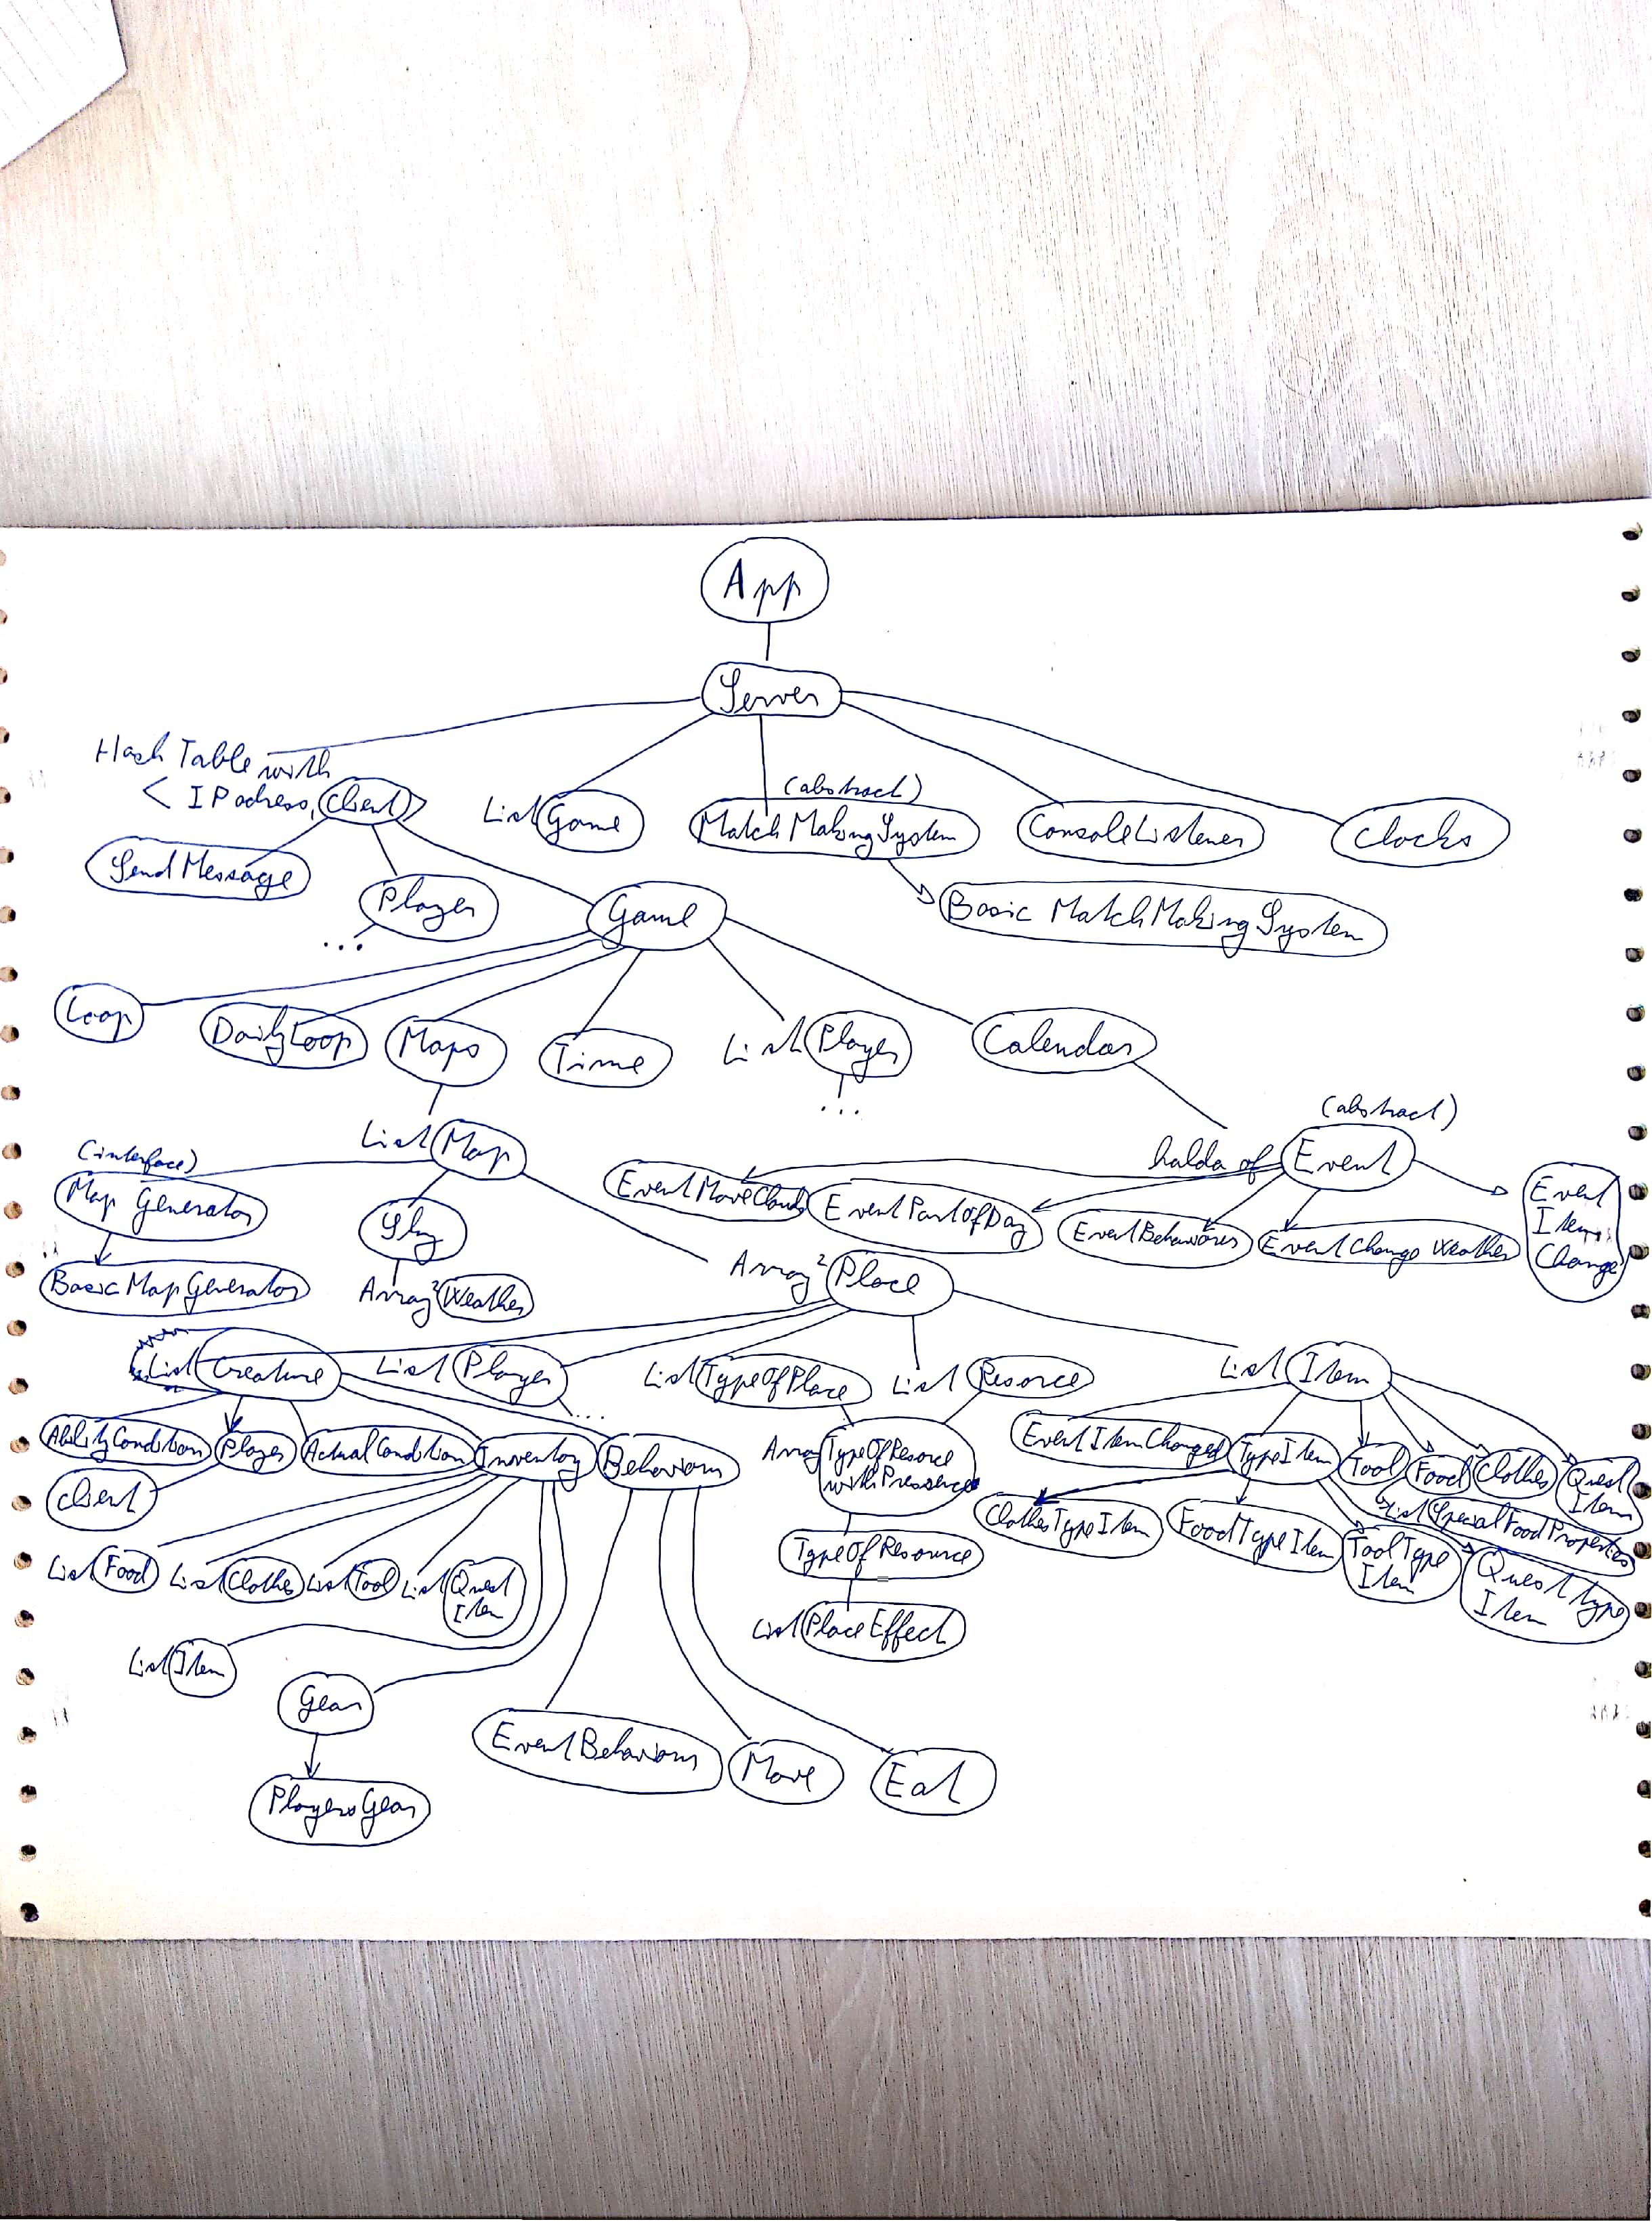
\includegraphics[width=\paperwidth]{objektovy_navrh.jpg}}
\end{center}
\section{App}
Obsahuje main metodu. V ní je vytvořen objekt Server.
\section{Objekt Server}
Tento objekt zajišťuje komunikaci s Klientem. Vytváří spojení a ukládá si informace o klientovy.

Obsahuje hashovací tabulku, kde klíčem je ip adresa klienta a obsahem je objekt Client.

Dále tento objekt obsahuje list objektů typu Game a nějaké další objekty viz obrázek.
 
\section{Clocks}
Obsahuje vedlejší vlákno, které řídí čas všech aktuálně běžících her. Běží v nekonečném loopu a k proměnné time přičítá jedničku, a pak se na určitou dobu uspí. Každá hra si pak pamatuje čas, kdy započala a pokud chce získat čas ve hře, odečte aktuální čas od času započetí hry.

\section{ConsoleListener}
Tato třída obsahuje vytváří nové vlákno, které sleduje text v konzoli, zda-li někdo do něj něco nenapsal. Provozovatel serveru pak může používat logy, které vypisují informace, které chce uživatel vědět. Pokud nenapíše log před zprávou, zpráva, kterou napíše je automaticky odeslána všem hráčům hry, která se v arraylistu her vyskytuje na nulté pozici.

\section{MatchMaking}
Tato třída je abstraktní, protože takových systémů může být hodně. Tato třída tedy obsahuje pouze interface metody, které potřebuje správný matchmaking systém. 

Tato třída je dále děděna prozatímním velmi jednoduchým BasicMatchMakingem, který pouze čeká na to, až spustit hru bude chtít dostatečně veliký počet hráčů, načež zahájí hru a čeká na novou várku hráčů.

Vytváří nové objekty game a přidává je do seznamu v Serveru.

\section{Client}
Tento objekt obsahuje informace o klientovy. Je zde například uveden jeho aktuální stav, jeho ip adresa, objekt SendMessage, který obsahuje metody na poslání zprávy klientovy, objekt aktuální hry, kterou zrovna hráč hraje (pokud nějakou hraje), dále jsou zde metody na obnovení připojení k serveru.

\section{Game}
Objekt obsahuje vše o jedné konkrétní hře. Kromě věcí napsaných v objektovém návrhu je zde např. stav hry, jestli je v přípravě, probíhá, nebo je ukončena. Obsahuje metody pro zahájení hry a vytvoření unikátní id pro eventy, předměty a creatury. 

\section{Time}
Obshauje statické metody pro převod jednotky času na minuty, dny, hodiny a další. Platí, že 20 tiků v Clocks (v serveru) je jedna hodina. Objekt pak obsahuje metody na zisk aktuálního času v dané hře.

\section{DailyLoop}
Neobsahuje nové vlákno, ale obsahuje pouze metody, které se zavolají, když končí den. V metodě nahází do kalendáře eventy typu EventPartOfDay. Říká to, kdy má dojít ke změně nového části dne. Tato informace je důležitá pro hráče, protože dle denní doby je ovlivněn barva filtru na pozadí před obrázkem.

\section{Loop}
Tato třída by se asi dala připodobnit k hlavnímu hernímu loopu. Jak název napovídá, jedná se o samostatné vlákno v nekonečném cyklu, dokud běží hra. Jediné co toto vlákno provádí je, že sleduje první nadcházející event v kalendáři a porovnává jeho datum s aktuálním časem hry. V případě, že nadešel čas eventu, zavolá se příslušná metoda objektu Event, který má nastat.

\section{Calendar}
Je to datová struktura, která obsahuje objekty Event, která vlastní hodnotu date, datum, kdy má k danému eventu dojít. 

Tato datová struktura pak musí umět ze všeho nejrychleji vyhledat event, který má nastat jak první ze všech v kalendáři. Dále je potřeba umět rychle odstraňovat tento první prvek.

\paragraph{}
Také je potřeba rychle (ale ne tak rychle jako dřívější operace) přidávat nové eventy, následně také vyhledávat eventy a nakonec rychle odstraňovat eventy, které se nachází uprostřed kalendáře.

\paragraph{}
Vymyslel jsem řešení, které pracuje v konstantním čase, jednalo by se o kombinaci spojového seznamu a "radix tree", stromu, kde uzly jsou číslo 0, nebo 1 (ukládám objekty dle data jako klíče, v kořenech je spojový seznam eventů). Hloubka takovéhoto stromu je délka čísla v binární soustavě...

Zde dochází k malinkému problému, nevím jak spočítat co by se vyplatilo. Pokud budu čísla do stromu ukládat v binární soustavě, vyhledávám selektováním jednotlivých  bitů bitovou maskou, což je velmi rychlé, na druhou stranu provádím více porovnání, než se dostanu do kořene. Pokud bych čísla ukládal v desítkové soustavě, uzel si bude zbytečně nechávat prostor pro zatím volné čísla a navíc při hledání objektu dle data provádím dělení a modulení pro selektění konkrétní číslice, což je extrémě pomalé. Přikláněl bych se tedy spíše, že rychlejší bude vyhledávání při zápisu čísla do stromu v binární soustavě.

\paragraph{}
Spojový seznam obsahuje ty samé objekty, každý objekt si pamatuje kde ve spojovém seznamu leží (ví přední i zadní prvek) a ví, kde ve stromě leží. 

Pak mohu provádět operaci zjištění, zda-li má nastat event, konstantní časovou složitost o jedničkové konstantě v podstatě. Odstranění prvního prvku by trvalo maximálně počet bitů data porovnání. Všechny ostatní operace v podstatě také. (teoreticky pokud by pod stejným klíčem data bylo hodně eventů naráz, pak pokud bych chtěl něco odstranit, nalezení by mohlo nejhůře trvat projití celého tohoto spojovém seznamu + nalezení ve stromě).

\paragraph{}
Problém je, že se to pro málo eventů tato implementace datové struktury nevyplatí, protože konstanta je příliš veliká. Jedná se o počet bitů data porovnání, což pokud si vezmu 2B číslo je 16 porovnání jen pro vyhledání 1 objektu. Přičemž počítám s tím, že porovnávat dva bity a dvě * 4B čísla je stejně zdlouhavé. 

Pro odstranění čísla navíc je potřeba projít strom v nejhorším případě 2x, tedy 32 porovnání, navíc datum je omezeno na 16 bitů, což je ve světě myslím jen několik měsíců. Tento problém by asi nevadil moc, ale přesto, pokud bych si vzal implementaci této datové struktury pomocí haldy, ověření vrchního eventu je instantní a ostatní trvají logaritmickou složitost, což když jsem si vypočítal je rychlejší než má implementace s konstantní časovou složitostí pro 1000 eventů. Více eventů než 1000 snad mít nebudu, takže jsem použil implementaci haldou.

\section{Event}
Event je abstraktní třída, která obsahuje společné metody action(), interrupt(), action provede akci eventu, interrupt znamená, že něco přerušilo event, takže k němu nedojde.
Z tohoto objektu je dále děděno.
\subsection{EventPartOfDay}
Pouze posílá klientům info o změně denní doby. Ráno a večer se posílá 2x a 2x info o sun rise a sun set, proto, aby se snadno měnil filtr na pozadí, protože u klienta pochopitelně dochází při změně denní doby k přechodu z 1 barvy do 2., tudíž u východu a západu slunce je potřeba v krátkém časovém úseku změnit barvu filtru rychleji.  

Vždy večer se do kalendáře nahází nové na celý den dopředu.

\subsection{EventItemChange}
Mění konkrétní staty předmětu, např. jídlo, že se má více zkazit.

\subsection{EventMoveClouds}
Tento event se podobně jako EventPartOfDay neustále opakuje s delayem dle síly větru. Posune s každým počasím nad daným políčkem mapy. 

Rafinovaně jsou Weather objekty každého políčka uloženy ve svém vlastním dvoudimenzionálním poli, kdy mám uloženy souřadnice = q (pro danou mapu), jaký objekt počasí se přiřazuje k políčku mapy na souřadnice [0;0]. Pokud mám konkrétní políčko mapy a chci zjistit počasí na něm, stačí k jeho pozici na mapě přičíst souřadnice q a modulit velikostí mapy a pak se podívat na příslušné souřadnice do pole objektů Weather. 

\paragraph{}
Pokud bych chtěl pohnout celou oblohou, stačí pouze pohnout q-čkem a na příslušných místech dogenerovat nové počasí. Časově mnohem méně náročné než procházet celou mapu a vše ručně posouvat.
\subsection{EventChangeWeather}
Provádí se pravidelně a mění počasí. Pomocí pravděpodobnosti se vyhodnotí, k jaké změně došlo. Nemusí se na daném políčku stát nic, nebo pokud jsou na políčku mraky, může začít pršet, přičemž platí, čím více mraků, tím větší pravděpodobnost, že začne pršet, a také tím větší pravděpodobnost, že bude větší bouřka. Také pokud už prší může přestat, nebo začít méně, podle toho, jak dlouho již prší. 

Bohužel zde musím procházet každé políčko Weather zvlášť.

\subsection{EventBehaviour}
Volá akorát příslušné metody v objektu Behaviour. action zavolá cease(), což je jakoby ukončení behaviour a interrupt zavolá interrupt().


\section{Maps}
Při vytvoření tohoto objektu je v konstruktoru naplněno pole objektů Map.

Tento objekt obsahuje akorát pole objektů Map.

\section{Map}
 Samotný objekt Map obsahuje objekt Sky, a dvoudimenzionální pole objektů Place.  

Při vytváření nové mapy v konstruktoru, je nutné předat daný generátor mapy MapGenerator, díky kterému je celá mapa nějak vygenerována.

Druhou variantou je při vytváření objektu Map konstruktoru předat cestu k souboru, kde je mapa uložena. Tato verze ovšem není zatím implementována.
 
\section{Sky}
Obloha obsahuje dvoudimenzionální pole objektů Weather a další vlastnosti oblohy, jako síla a směr větru, nebo souřadnice počátku, který Weather se zobrazí na Place pozice [0;0]. Dále jsou zde metody na pohyb a změnu mraků, počasí.

\section{Weather}
Objekt obsahuje vlastnosti počasí, tedy počet mraků na obloze od 0 do 5, síla deště od 0 do 6 a doba, jakou už prší, čím větší, tím větší pravděpodobnost, že přestane pršet.

\section{MapGenerator}
Je to interface, který pouze implementuje metody pro nastavení počasí a nastavení všech políček Place.

Mohu si tak udělat jak generátor přírody, tak generátor na úplně cokoli jiného.

\section{BasicMapGenerator}
Implemntuje MapGenerator, přičemž u počasí, nejprve vygeneruje v prvním sloupci a řádku celého dvoudimenzionálního pole Weather, a následně generuje mraky, kdy pokud se nalevo a nad ním nachází také mrak, pravděpodobnost, že na novém políčku bude také mrak je vyšší.

Samotné Places se vygeneruje tak, že nejprve se vezme primitivní mapa, což je mapa, která rozdělí celou mapu na jednotlivé bloky (2x2), a každému se následně přiřadí interval nadmořské výšky, přičemž při generování nadmořské výšky se podívám na okolní políčka a jejich nadmořskou výšku, vypočítám jejich aritmetický průměr a náhodně vyberu, jestli se změní hodnota o jeden interval nahoru, nebo dolu, nebo jestli zůstane na průměru. Nadmořská výška je interval mezi 0 až 1000, ten je rozdělen na 5 podintervalů po 200, protože na každém podintervalu se vyskytují jiné typy míst. 

\section{Place}

Tento objekt obsahuje veškeré informace o konkrétním políčku mapy. Obsahuje informace, jako jaké creatury se zde vyskytují, jaké předměty, přírodní bohatství políčka (co se zde dá nalézt), obrázek, který se má zobrazit na pozadí, hudba, která se má přehrávat a také objekt TypeOfPlace.

Navíc ještě obsahuje list s objekty PlaceEffect.
\subsection{temperature}
Teplota se vypočítává u daného místa, kdy je potřeba.

Chová se lineárně v závislosti na nadmořské výšce, přičemž v nule je teplota 30.

Dále je ovlivněna aktuálním počasím, pokud mapa má oblohu.

\begin{verbatim}
    public int getTemperature() {
        int temperature = 30 - (altitude / 80);
        if(map.sky != null){
            Weather weather = map.sky.getWeather(this);
            temperature -= weather.getClouds();
            temperature -= weather.getWeather();
        }
        return temperature;
    }
\end{verbatim}

\subsection{Visibility}
\subsubsection{getVisibility()}
Vrací hodnotu viditelnosti na daném políčku. Je ovlivněno hodnotou visibility daného place a visibility daného weather (která se posouvá silou větru).
\begin{itemize}
\item 
Visibility počasí může být například mlha. Něco co brání v dohledu, ale zároveň se to posouvá silou větru.
\item
Visibility v place je ovlivněno nápadností resources nacházejících se zde. Vypočítám si 
\end{itemize}
\section{TypeOfPlace}
Tento objekt shrnuje všechny informace společné pro daný typ políčka. Například políčko listnatý les bude mít podobné vlastnosti jako jiné políčko listnatý les. Každé place, které má být listnatým lesem, má stejný objekt TypeOfPlace. Tyto objekty jsou definovány ve třídě ListOfAllTypesOfPlaces, která obsahuje statické pole všech možných TypeOfPlace. K nastavení jich dochází při zapnutí aplikace ještě před vytvořením prvního serveru.

\paragraph{}
TypeOfPlace obsahuje pole obrázků, které jsou typické pro daný typ místa, pole písniček, které jsou typické pro dané místo, obsahuje také pole int čísel, které říkají v jaké nadmořské výšce se může daný typ políčka vyskytovat.

Pole TypeOfResourceWithPressence říká, jaké typy resourců (přírodního bohatství) se zde může vyskytovat a s jakou pravděpodobností se zde vyskytuje.

\section{Resource}
Jelikož během hry nemá v podstatě žádné dynamické vlastnosti, obsahuje zatím pouze objekt TypeOfResourceWithPressence. 

\subsection{speedOfFinding}
Každá resource má svou vlastní hodnotu durationOfFinding, která říká, jak dlouho trvá, než je nalezena. Tato hodnota se nastavuje po vytvoření daného resource v Place, přičemž je nastavena podle ostatních resource, čím více lépe viditelných resource se zde nachází, tím hůře půjde tato resource nalézt.

Při nastavení těchto hodnot se tedy musí setřídit všechny resource na daném place podle hodnoty conspicuousness v TypeOfResource. Následně postupně procházím od resource s nejvyšší nápadností, u ní bude vyšší rychlost nalezení (pochopitelně první resources budou pravděpodobně nalezitelné instantně). 

Čím větší nápadnost, tím více zakrývá ostatní resources s menší nápadností.

Resources se stejnou conspicuousness se navzájem neovlivňují, ale dohromady více ovlivňují resources s menší conspicuousness než jako kdyby se počítali dohromady jako 1 resource.

\subsubsection{get durationOfFinding} 
Hodnota durationOfFinding se vypočítává z hodnot durationOfFinding daného typu resourceru a hodnoty amount, která je uložena přímo v resourceru. Amount říká, kolik se daného resourceru na place nachází. Hodnota 100 znamená 100 procent, a tím pádem durationOfFinding je rovna hodnotě durationOfFinding z typu resourceru.

Hodnota amount je z počátku nastavena dle hodnoty startAmount, která je v ResourcesWithPressence (tedy pro každý typeOfResource může být jiná).

\subsubsection{set amount, nebo durationOfFinding}   
po změně

\subsubsection{hodnoty}

\begin{itemize}
\item{conspicuousness} $0 ... 2^{31}$ Chceme, aby conspicuousness bylo neomezené na maximum nápadnosti, min může být. 0 tedy znamená nulová nápadnost a nižší už být nemůže, čím vyšší, tím vyšší nápadnost, nejlépe lineární chování.

\item{durationOfFinding}
$0...2^{31}$, kde 0 je instantní nalezení a n je čekání n tiků ($n * 3$ minuty).
\end{itemize}

\subsubsection{výpočet durationOfFinding}
Procházíme seřazené resources. První je nejlépe vidět, \textbf{musí být viděn instantně}, tedy hodnota je nula.

Hodnota u následující je ovlivněna velikostí consp. hodnotou. Čím větší je rozdíl v consp., tím více ovlivní, resp. zvýší durationOfFinding value aktuální. $a_1=c_0-c_1$
$$ a_k=\sum_{i=0}^{k-1} (c_i-c_k)= \sum_{i=0}^{k-1} c_i-c_k*k$$

\subsubsection{Pozorování}
Nechová se dokonale v případě, kdy na daném place je spousta resources s podobnou consp., protože creatura přesto ihned uvidí resource s nejvyšší consp.

\subsubsection{výpočet durationOfFinding, když v place resource není}

Provádí metoda getDurationOfFindingOfResourceWhichIsNotHere() ve třídě Place. Prochází se setříděné pole resourců daného place, sčítají se postupně jednotlivé conspicuousness daných place. To se porovnává s hodnotou conspicuousness s hodnotou 50 amount, tedy se counspicuousness vydělí 2, hledaného resource. 

\subsection{Skupiny}
\subsubsection{motivace}
Chceme mít možnost rozdělení resources do skupin, přičemž každá skupina si bude moct nastavit vlastní pravidla. Může se jednat právě například o skupinu resources rostliny rostoucí v přírodě, nebo mix typů stromů rostoucí v přírodě, tak aby dohromady nezvyšovaly neprůhlednost v place.

U rostlin je potřeba mít u každé rostliny vlastní hodnotu rychlosti nalezení, zároveň ovšem chceme creatuře umožnit, aby mohla hledat obecnou rostlinu. Pro to potřebujeme společnou hodnotu doby hledání a následně algoritmus pro výběr nalezené rostliny (pro rostliny pravděpodobně pomocí náhody). 

\subsubsection{implementace}
Chceme umožnit co nejobecnější přístup, aby následná implementace mohla zahrnovat co nejvíce možností použití.
Pro hledání konkrétních resources se tedy přidá zvlášť do seznamu resourců daného place. Pro hledání skupiny resourců se použije externí kód běžící mimo. Objekt skupina resourců obsahuje skupinu typů resourců a vlastní metodu pro vybrání nějakého resourcu při objevení. Pro každou place bude muset počítat zvlášť. Musí se vzít průnik množin resourců v place a v skupině typu resourců. Pokud creatura daný resource nalezne, přidá se u příslušného resource CreatureKnowsAboutResource.

\section{TypeOfResource}
Obsahuje název resource a rychlost, jak snadno lze daný Resource nalézt. Je rozšířen objektem TypeOfResourceWithPressence, který obsahuje objekt TypeOfResource a pravděpodobnost výskytu na daném typu místa.

Obsahuje také pole tzv. PlaceEffect

\section{PlaceEffect}
Jedná se o efekt, který by mohl být viděn z okolních políček. Například, pokud by někde docházelo k požáru, kouř bude vidět z okolních políček.

\section{Creture}
Stvoření je základ pro všechno co se pohybuje po světě.  

\paragraph{}
Obsahuje objekt ActualCondition, AbilityCondition, Behaviour s jeho aktuální činností, dále Inventory a pak jen id a vzhled.

\section{Player}
Dědí z Creature a jedná se o hráče připojené přes server.
\section{Condition} 
\subsection{ActualCondition}
Obsahuje informace o aktuálním stavu hráče. Jde o hodnoty zdraví, hladu, únavy, teploty, pozornosti... Hodnoty, které se mohou postupně měnit časem. Každá vlastnost zde má svůj EventCreatureActualCondition, který se vkládá do kalendáře. A postupně se hodnota vlastnosti snižuje. 

Hodnota vlastnosti nabývá od 100 do 0.

\paragraph{HeatEvent}
Hodnota se mění pravidelně jednou za čtvrt hodiny, tedy za 15 tiků.

Hodnota se snižuje, pokud je okolní teplota menší jak 23 stupňů. Pokud je teplota naopak vyšší, hodnota se zvyšuje. 
Rychlost tepelné výměny závisí na hmotnosti m, velikosti povrchu S, rozdílu teplot $\Delta t$, měrné tepelné kapacitě c, součinitel tepelné vodivosti k (rychlost předání tepelné energie na povrchu mezi 2 prostředími).   
$$ v = \frac{S \Delta t k}{m c} $$

$$  Q = \frac{\Lambda \tau S \Delta t}{d} $$

Povrch je konstantní, součinitel tepelné vodivosti a měrná tepelná kapacita také. 

$$ v \in O(\frac{\Delta t}{m})$$

v je v jednotkách stupně celsia za vteřinu.

\subsection{AbilityCondition}
Obsahuje všechny vlastnosti, které se nemění kvůli prostředí, ve kterém kreatura je.

Hodnoty síly, hbitosti, zraku, vytrvalosti...

\section{Item}
Obsahuje informace o konkrétním předmětu, přímo tedy obsahuje hodnoty, které jsou různé pro každý předmět. Je to například Creature, neboli vlastník předmětu, typ předmětu a EventItemChange, přičemž obsahuje také metodu changeStats().

Následující skupiny dědí z Item:

\subsection{Food}
Obsahuje specifické vlastnosti pro konkrétní jeden předmět typu food. To je například teplota jídla, míra čerstvosti. 
Dále má dva EventItemChange, které mění časem ony hodnoty.

Dále je zde list SpecialFoodsProperties, které říkají jaké speciální vlastnosti předmět má (jaké hodnoty hráče po snězení mění).

\subsection{Clothes}
Obsahuje informace o špinavosti, ostatní vlastnosti jsou stejné pro daný typ oblečení.

\subsection{Tool}
Jediná value kvalita nástroje.

\subsection{QuestItem}
Na tom zatím nepracuji.

\section{TypeItem}
Každý item má definovaný svůj typeItem, kdy každý item stejného typu vlastní odkaz na stejný typ předmětu. Tato třída tedy obsahuje informace, které jsou typické pro daný typ.

Jsou definovány ve statickém poli v ListOfAllItemTypes.

Následující třídy dědí z TypeItem:

\subsection{FoodTypeItem}
Hodnoty rychlosti kažení, míry zaplnění po snědení. Pole SpecialFoodProperties, název jídla.

\subsection{ClothesTypeItem}
Hlasitost, zateplení, obrana před nárazy, ovlivnění viditelnosti, definování typ oblečení (kalhoty, čepice, bunda...).

\subsection{ToolTypeItem}
Rychlost poškození používáním, jméno.


\section{Inventory}
Zde se ukládají předměty, které hráč vlastní. Gear pak říká jaké oblečení má na sobě creatura.

\section{Behaviour}
Je abstraktní metoda, obsahuje metody jako execute(), započení aktivity, interrupt(), přerušení, case(), ukončení.

Má hodnoty dobu trvání, náročnost úkonu, EventBehaviour.

Každý typ činnosti dědí z Behaviour.

Zatím máme činnost Move, kdy se creatura začne pohybovat po mapě, a Eat, kdy creatura sní nějaký předmět typu Food.

\subsection{FindConcreteResource}
Pokud se daný typ Resource na Place nenachází, vypočítám si jakou by resource mělo durationOfFinding, kdyby se zde nacházelo. V place využiji seřazené pole všech resources dle nápadností a sečtu všechny rozdíly nápadností a nápadnosti našeho typeOfResource, kromě nižších nápadností. Takovou dobu pak musí creatura hledat, než zjistí, že zde daný resource není.

\section{CreatureMemory}
Každá creature si bude muset pamatovat všechny informace, se kterými přišla do kontaktu. Může to být například informace, kde leží daný předmět, kde na políčku se nachází dané resource.

\chapter{Client}
Bohužel u klientské aplikace jsem nestihl naprogramovat to co jsem si vytyčil. Funguje pouze spojení se serverem a zapnutí hledání hry, kdy hráč na serveru vstoupí do match makeingu. 

\paragraph{}
Samotná aplikace je zahájena zapnutím MainActivity. Tato aktivita je v podstatě prázdná. Ověřují se zde počáteční základní informace, jako například zda-li je aplikace spuštěna poprvé. Aktivita může zobrazovat například nějaké logo.

Následně aktivita zapne novou aktivitu. Pokud je aplikace zapnuta poprvé, je zapnuta tzv. WelcomingActivity, v případě, že není, zapne se rovnou MenuAktivity.

Menu aktivity nejprve zobrazí ConnectToServerFragment, které obsahuje formulář pro připojení se k danému serveru pomocí ip adresy a portu. V OnCreate() se také vyzkouší uložné hodnoty minulého připojení k serveru, aby nebylo třeba to psát pokaždé znovu.

\chapter{Závěr}
\section{Klient}
Výsledná klientská aplikace by měla být obohacena o GameActivity, která se zapne po spuštění hry. Na pozadí se bude nacházet ImageView, který obsahuje obrázek aktuálního Place, na kterém se hráč právě nachází. Před ním se pak nachází View s průhledným background. Toto background mění svou barvu a průhlednost dle aktuálního úseku dne (zda-li je ráno, večer, noc...). 

Dále toto View mění svou barvu podle aktuálního velikosti mraku na obloze. Čím větší mrak, tím tmavější a méně průhledný by View mělo být. Navíc, pokud bude mrak dostatečně malý, mělo by se spustit nové vlákno, které bude zařizovat, aby se obloha zatmavila na krátkou chvíli a pak zase rozjasnila. 

Před tímto view se dále nachází fragment, který je průhledný, a který obsahuje uživatelské rozhraní. Těchto fragmentů je více a každý obsahuje to, k čemu je určen. Tímto fragmentem může být například inventář, aktuální stav hráče, mapa (co hráč aktuálně vidí okolo sebe), behaviour fragment, kde může hráč provádět behaviours, nebo fragment chat, pro komunikaci s okolními creatures, které jsou na stejném políčku.

\paragraph{}
Je potřeba opravit některé chyby. Například, když se uživatel nachází v menu a uspí mobil, po znovu otevření aplikace spadne. Problém je v znovu naplnění fragmentu, přesný důvod zatím nevím.

\section{Server}

Server je sice relativně dobře provedený nyní, přesto je ještě spousta věcí, které bude potřeba přidělat. Příkladem může být změna hráčových vlastností, jako je hlad, teplota, únava...

\subparagraph{}
Potřeba je také opravit jednu menší chybičku u Kalendáře.

%%% Prostor pro přílohy práce
\chapwithtoc{Přílohy}
Zde přikládám odkaz na můj kód:

\url{https://gitlab.mff.cuni.cz/teaching/nprg031/2021-summer/student-tichavso.git}

\openright
\end{document}
